\begin{figure}
  \centering

  \begin{subfigure}[t]{0.49\textwidth}
    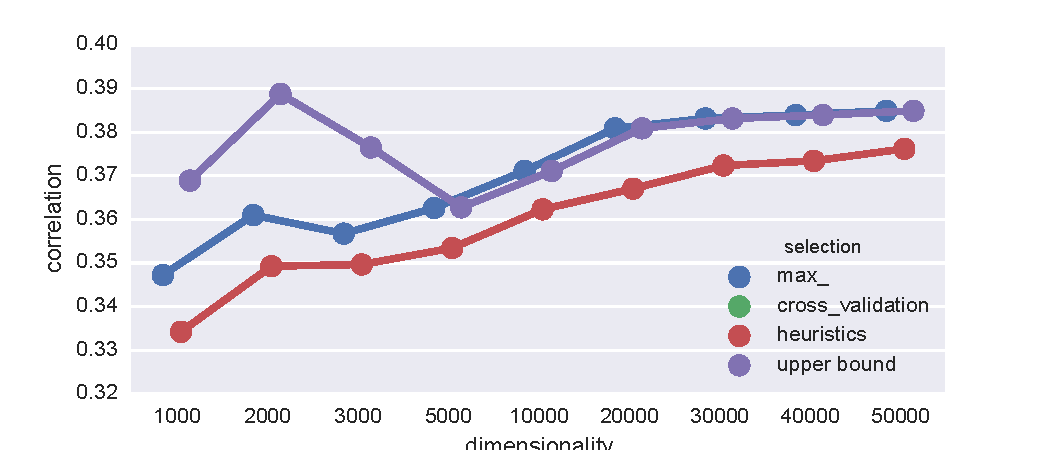
\includegraphics[width=\textwidth]{supplement/figures/lexical-results-SimLex999}
    \caption{SimLex-999.}
    \label{fig:lexical-results-simlex}
  \end{subfigure}
  \begin{subfigure}[t]{0.49\textwidth}
    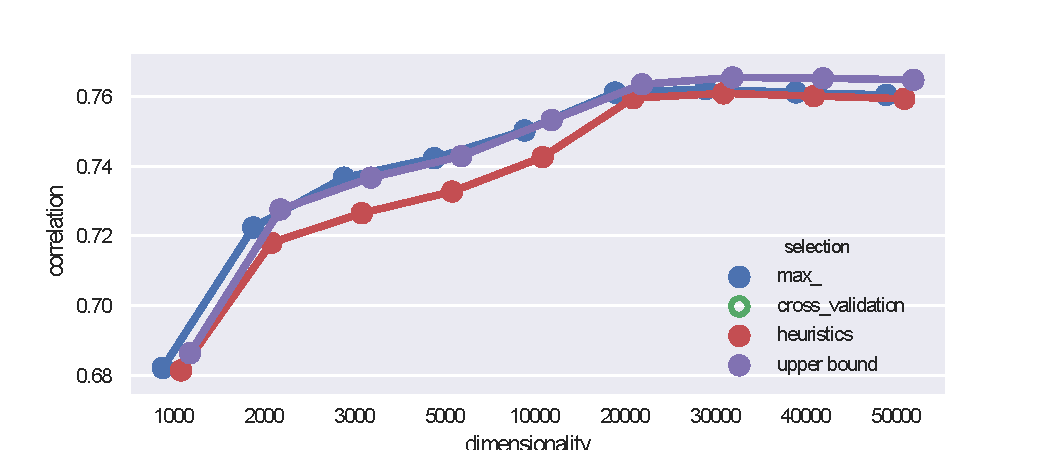
\includegraphics[width=\textwidth]{supplement/figures/lexical-results-men}
    \caption{MEN.}
    \label{fig:lexical-results-men}
  \end{subfigure}

  \caption{Performance of models based on the selection over the average lexical performance}
  \label{fig:lexical-results}
\end{figure}

%%% Local Variables:
%%% mode: latex
%%% TeX-master: "../thesis"
%%% End:
